\chapter{Análisis del problema}

Como hemos comentado en el anterior capítulo, la principal competencia actual está 
bastante anticuada, especialmente en el ámbito de los memes.
\\\\
Para convertir este proyecto en algo viable y competitivo, deberemos asegurarnos de que
el usuario tenga una experiencia fluída, en contraposición con el resto de editores.
\\\\
Una de las principales carácterísticas que debe tener es poder cargar, editar y subir sin
necesidad de descargar nada en ningún momento.
\\\\
El editor debe ser simple y rápido, cargar rápido, responder rápido
y, en general, resaltar en la medida de lo posible en todos los aspectos 
que fallan en los editores locales convencionales.
\\\\
Además otro de los objetivos del proyecto es la posibilidad de llevar a 
cabo todo esto manteniendo al servidor libre de carga, ya que, los cálculos
y las ediciones sobre contenido multimedia consume bastante capacidad de 
procesamiento y de red ya que tendríamos que enviar el multimedia al servidor.
\\\\
Lo mas lógico por ende para solucionar esto es hacer que la aplicación sea 
puro front-end, es decir, emplear un esquema donde el servidor se desentiende
tras enviar el software que se ejecute en el navegador.
\\\\
Para este tipo de aplicaciones está bastante generalizado el uso de frameworks 
y bibliotecas front-end como Vue.js o React.js.
\\
Tras investigar y comparar las diferentes posibilidades finalmente nos decantamos
por el uso de React.js ya que era el framework que mejor permitía dar
la experiencia de usuario que deseamos, una aplicación reactiva, donde tenemos
un gran control sobre el rendimiento durante el desarrollo gracias al 
desarrollo enfocado a componentes de React.js que nos permitirá actualizar
en cada momento sólo algunas partes de la aplicación.  
\\\\
Tras la elección de la biblioteca que vamos a utilizar.
hemos planteado que el editor esté formado por las siguientes partes:

\begin{figure}[!h]
    \centering
    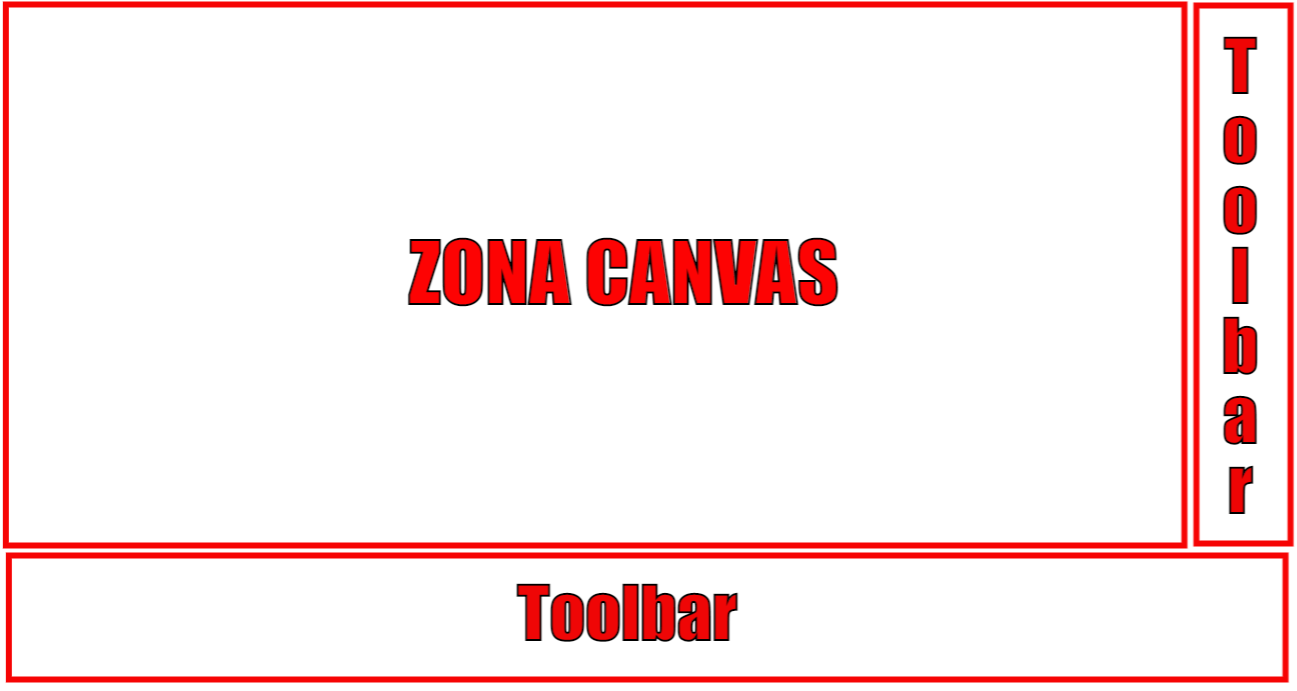
\includegraphics[scale=0.30]{img/ESQUEMA_ABSTRACTO.png}
    \caption{Esquema de las partes que debería tener el editor}
\end{figure}

Como vemos es una estructura simple, con partes claras y diferenciadas, 
que tiene en cuenta todos los objetivos planteados anteriormente.